\documentclass[]{article}
\usepackage{amsmath}
\usepackage{amssymb}
\usepackage{graphicx}
\usepackage{subfig}
\graphicspath{{./imgs/}}
%opening
\title{Normalizing Flows}
\author{Abdul Fatir}
\date{}
\begin{document}

\maketitle

\begin{abstract}
Notes on normalizing flows.
\end{abstract}

\section{Introduction}
Simple distributions (e.g., Gaussian) are often used as likelihood distributions. However, the true distribution is often far from this simple distribution and this results in issues such as blurry reconstructions in the case of images. Latent variable models such as VAEs often set the prior distribution $p(\mathbf{z})$ to a factorial multivariate Gaussian distribution. Such a simplistic assumption hampers the model in multiple ways. For instance, this does not allow a multi-modal latent space distribution. Normalizing Flows allow transformation of samples from a simple distribution (subsequently denoted by $q_0$) to samples from a complex distribution by applying a series of invertible flows.

\subsection{Distribution of a Simple Transformation of a RV}

Before jumping into normalizing flows, let's consider a simple univariate distribution $p(x)=2x$ with support $x\in[0,1]$. Define a function $y = f(x) = x^2$. Note that $f(x)$ is monotonically increasing in $[0,1]$. What is the PDF of the variable $y$?

We can compute $p(y)$ using the CDFs as follows.

\begin{align}
F_{Y}(y) &= P(Y \leq y)\\
&= P(X^2 \leq y)\\
&= P(X \leq \sqrt{y})\\
&= F_{X}(\sqrt{y})
\end{align}

Now, $p(y) = F_{Y}'(y) = \frac{dF_{X}(\sqrt{y})}{dy}$ where

\begin{align}
F_{X}(\sqrt{y}) &= \int_{0}^{\sqrt{y}} p(x) dx\\
&=\left[2\frac{x^2}{2}\right]_{0}^{\sqrt{y}}\\
&=y
\end{align}

differentiating w.r.t. $y$ we get $\frac{d(y)}{dy} = 1$ which means that $p(y) = \mathcal{U}(0,1)$.

\subsection{Change of Variables}

The method described above can be extended to multivariate distributions $q_0(\mathbf{z})$ and smooth invertible mappings $f: \mathbb{R}^d\Rightarrow\mathbb{R}^d$. Samples $\mathbf{z} \sim q_0(\mathbf{z})$ can be transformed using $f$ to give $\mathbf{y}=f(\mathbf{z})$. The PDF of $\mathbf{y}$ is given by 

\begin{align}
q_1(\mathbf{y}) = q_0(\mathbf{z})\left|\det \frac{\partial f^{-1}}{\partial \mathbf{y}}\right| = q_0(\mathbf{z})\left|\det \frac{\partial f}{\partial \mathbf{z}}\right|^{-1}
\label{eq:cov}
\end{align}

where the second equality comes from the inverse-function theorem.

Rezende et. al. proposed two different families of invertible transformations: planar flow and radial flow.

\section{Planar Flow}

Planar flows use functions of form


\begin{align}
f(\mathbf{z}) = \mathbf{z} + \mathbf{u}h(\mathbf{w}^\top\mathbf{z} + b)
\label{eq:planarfn}
\end{align}


where $\mathbf{u},\mathbf{w}\in \mathbb{R}^d$, $b \in \mathbb{R}$, and $h$ is an element-wise non-linearity such as $\tanh$.

The Jacobian is then given by

\begin{align*}
\frac{\partial f(\mathbf{z})}{\partial \mathbf{z}} = \mathbf{I} + \mathbf{u}h'(\mathbf{w}^\top\mathbf{z} + b)\mathbf{w}^\top
\end{align*}

Now, using the matrix determinant lemma

\begin{align}
\det\frac{\partial f(\mathbf{z})}{\partial \mathbf{z}} &= (1 + h'(\mathbf{w}^\top\mathbf{z} + b)\mathbf{w}^\top\mathbf{I}^{-1}\mathbf{u})\det(\mathbf{I})\\
&=(1 + h'(\mathbf{w}^\top\mathbf{z} + b)\mathbf{w}^\top\mathbf{u})\label{eq:planar-det}
\end{align}


\subsection{Example}

Let's look at a specific example for $\mathbf{z}\in\mathbb{R}^2$. We will apply a planar flow to $\mathbf{z}$ to get $\mathbf{y} = f(\mathbf{z})$.


\begin{align*}
q_0(\mathbf{z}) &= \mathcal{N}(\mathbf{z};\mathbf{0},\mathbf{I})\\
\mathbf{w} &= \begin{bmatrix}5 & 0\end{bmatrix}^\top\\
\mathbf{u} &= \begin{bmatrix}1 & 0\end{bmatrix}^\top\\
b &= 0\\
h(\mathbf{x}) &= \tanh(\mathbf{x})
\end{align*}

The determinant of the Jacobian can be computed using Eq. ($\ref{eq:planar-det}$) and the analytic PDF $q_1(\mathbf{y})$ can then be computed using Eq. ($\ref{eq:cov}$). The effect of the flow on uniformly space points is shown in Figure \ref{fig:planar-points}. The analytic density $q_0(\mathbf{z})$ and the corresponding empirical density plotted as a 2D histogram of samples from $q_0(\mathbf{z})$ is shown in Figure \ref{fig:q0}. The analytic density $q_1(\mathbf{y})$ computed using Eq. ($\ref{eq:cov}$) and the corresponding empirical density plotted as a 2D histogram of variables $\mathbf{y}$ obtained by applying $f$ to samples from $q_0(\mathbf{z})$ is shown in Figure \ref{fig:q1-planar}.

\begin{figure}
		\centering
	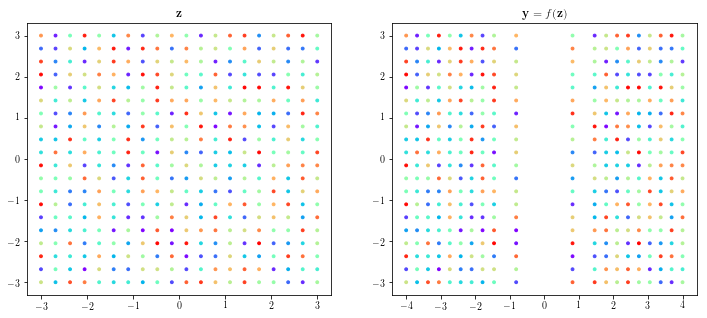
\includegraphics[width=0.6\textwidth]{planar-points}
	\caption{Applying planar flow to uniformly spaced points}
	\label{fig:planar-points}
\end{figure}

\begin{figure}
		\centering
	\subfloat{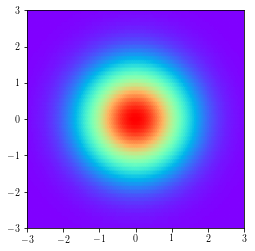
\includegraphics[width=0.3\textwidth]{planar-q0}}
	\subfloat{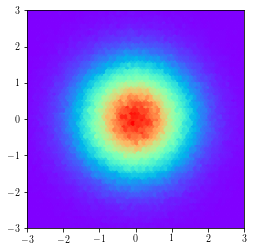
\includegraphics[width=0.3\textwidth]{planar-q0-emp}}
	\caption{Analytic and empirical density $q_0(\mathbf{z})$}
	\label{fig:q0}
\end{figure}

\begin{figure}
	\centering
	\subfloat{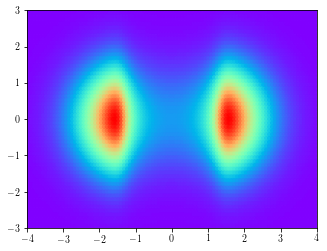
\includegraphics[width=0.3\textwidth]{planar-q1}}
	\subfloat{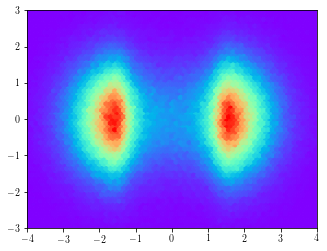
\includegraphics[width=0.3\textwidth]{planar-q1-emp}}
	\caption{Analytic and empirical density $q_1(\mathbf{y})$ after applying planar flow}
	\label{fig:q1-planar}
\end{figure}

\section{Radial Flow}
Radial flows use functions of the form

\begin{align*}
f(\mathbf{z}) = \mathbf{z} + \beta h(\alpha,r)(\mathbf{z}-\mathbf{z}_0)
\label{eq:radialfn}
\end{align*}

where $\alpha \in \mathbb{R}^+$, $\beta \in \mathbb{R}$, $h(\alpha,r) = (\alpha + r)^{-1}$ and $r = \vert\vert\mathbf{z} - \mathbf{z}_0\vert\vert$.

The Jacobian is then given by

\begin{align*}
\frac{\partial f(\mathbf{z})}{\partial \mathbf{z}} &= \mathbf{I} + \beta\left((\mathbf{z}-\mathbf{z}_0)h'(\alpha,r)\frac{\partial r}{\partial \mathbf{z}} + h(\alpha,r)\mathbf{I}\right)\\
&=(1+\beta h(\alpha,r))\mathbf{I} + \beta h'(\alpha,r)(\mathbf{z}-\mathbf{z}_0)\frac{(\mathbf{z}-\mathbf{z}_0)^\top}{||\mathbf{z}-\mathbf{z}_0||}
\end{align*}


Let $\gamma = (1+\beta h(\alpha,r))$. Again, using the matrix determinant lemma

\begin{align}
\det\frac{\partial f(\mathbf{z})}{\partial \mathbf{z}} &= \left(1 + \beta h'(\alpha,r)\frac{(\mathbf{z}-\mathbf{z}_0)^\top}{||\mathbf{z}-\mathbf{z}_0||}\frac{\mathbf{I}}{\gamma}(\mathbf{z}-\mathbf{z}_0)\right)\det(\gamma\mathbf{I})\\
&=\left(\frac{1 + \beta h(\alpha,r) + \beta h'(\alpha,r)||\mathbf{z}-\mathbf{z}_0||}{(1+\beta h(\alpha,r))}\right)(1+\beta h(\alpha,r))^d\\
&=\left(1 + \beta h(\alpha,r) + \beta h'(\alpha,r)r\right)(1+\beta h(\alpha,r))^{d-1}\label{eq:radial-det}
\end{align}

\subsection{Example}

Let's look at a specific example for $\mathbf{z}\in\mathbb{R}^2$. We will apply a radial flow to $\mathbf{z}$ to get $\mathbf{y} = f(\mathbf{z})$.


\begin{align}
q_0(\mathbf{z}) &= \mathcal{N}(\mathbf{z};\mathbf{0},\mathbf{I})\\
\mathbf{z}_0 &= \begin{bmatrix}1 & 0\end{bmatrix}^\top\\
\alpha &= 2\\
\beta &= 5
\end{align}

The determinant of the Jacobian can be computed using Eq. ($\ref{eq:radial-det}$) and the analytic PDF $q_1(\mathbf{y})$ can then be computed using Eq. ($\ref{eq:cov}$).  The effect of the flow on uniformly space points is shown in Figure \ref{fig:radial-points}. The analytic density $q_0(\mathbf{z})$ and the corresponding empirical density plotted as a 2D histogram of samples from $q_0(\mathbf{z})$ is shown in Figure \ref{fig:q0}. The analytic density $q_1(\mathbf{y})$ computed using Eq. ($\ref{eq:cov}$) and the corresponding empirical density plotted as a 2D histogram of variables $\mathbf{y}$ obtained by applying $f$ to samples from $q_0(\mathbf{z})$ is shown in Figure \ref{fig:q1-radial}.

\begin{figure}
	\centering
	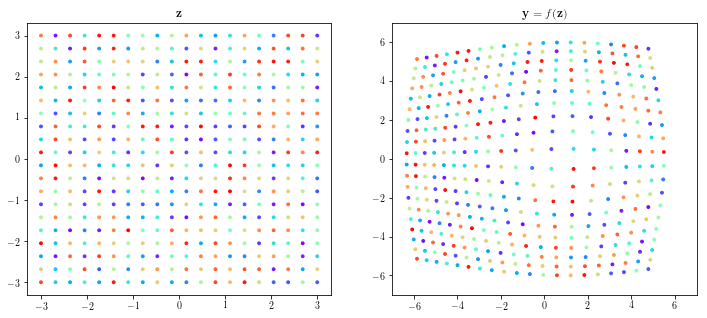
\includegraphics[width=0.6\textwidth]{radial-points}
	\caption{Applying radial flow to uniformly spaced points}
		\label{fig:radial-points}
\end{figure}

\begin{figure}
	\centering
	\subfloat{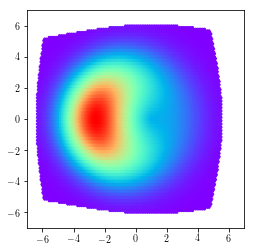
\includegraphics[width=0.3\textwidth]{radial-q1}}
	\subfloat{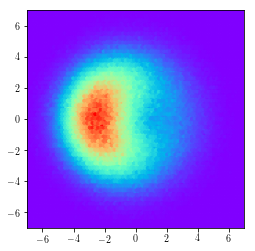
\includegraphics[width=0.3\textwidth]{radial-q1-emp}}
	\caption{Analytic and empirical density $q_1(\mathbf{y})$ after applying radial flow}
		\label{fig:q1-radial}
\end{figure}



\end{document}
